\documentclass[a4paper,oneside,12pt]{amsart}

%\usepackage[spanish, activeacute]{babel}
\usepackage[utf8]{inputenc}
%\usepackage[latin1]{inputenc}
\usepackage{latexsym}
\usepackage{multicol}
\usepackage{enumerate}
\usepackage{enumitem}
\usepackage[heightrounded]{geometry}
\geometry{top=2cm,bottom=2cm,left=2cm,right=2cm}
\usepackage{graphicx}
\usepackage{tikz}
\usepackage{amssymb}
\usepackage{tikz-network}

\DeclareMathOperator{\cond}{cond}
\DeclareMathOperator{\Id}{Id}
\DeclareMathOperator{\re}{Re}
%\DeclareMathOperator{\im}{Im}
\newcommand{\I}{\mathbb{I}}
\newcommand{\R}{\mathbb{R}}
\newcommand{\Q}{\mathbb{Q}}
\newcommand{\C}{\mathbb{C}}
\newcommand{\Z}{\mathbb{Z}}
\newcommand{\N}{\mathbb{N}}
\DeclareMathOperator{\im}{Im}

\newcommand{\nombremateria}
{Investigaci\'on Operativa}
\newcommand{\nombrecuatrimestre}
    {Segundo cuatrimestre de 2022}
\newcommand{\numeroparcial}
    { Recuperatorio del Tercer Parcial }
\newcommand{\fecha}
    {28 de Diciembre de 2022}
\newcommand{\numerotema}
    {\bf 1}

%\oddsidemargin -1cm \evensidemargin -1cm \textwidth 17.5cm
%topmargin 1.2cm \textheight 25cm
%\setlength{\textheight}{25cm}

\def \ds{\displaystyle}
\theoremstyle{definition}
\newtheorem{quest}{Ejercicio}
\thispagestyle{empty}

\begin{document}

\hfill \hfill
\begin{tabular}[c]{|c|c|c|c|c|}
\hline 
1 & 2 & 3 & 4 & Calificaci\'on \\ \hline \hline
\hspace{1.2 cm} & \hspace{1.2 cm} & \hspace{1.2 cm} & \hspace{1.2 cm}  &\hspace{1.5 cm} \\
\hspace{1.2 cm} & \hspace{1.2 cm} & \hspace{1.2 cm} & \hspace{1.2 cm}  &\hspace{1.5 cm} \\ \hline

\end{tabular}

\vspace{-1cm}

\noindent Nombre y apellido:

\vspace{0.2cm}

\noindent Número de libreta:

\noindent \hrulefill 

\smallskip
\renewcommand{\baselinestretch}{1.1}

\begin{center}
	\large \textbf{\nombremateria} 
	
	\numeroparcial -- \fecha
\end{center}

\noindent\textit{Para aprobar el parcial deberá obtenerse un puntaje mayor o igual que 4. \textbf{Entregue todos los ejercicios en hojas separadas.}}

\vspace{.6cm}
\renewcommand{\theenumi}{\textbf{\arabic{enumi}}}

%%% EMPIEZA EL EJERCICIO 1 %%%

\begin{quest}\verb|[3 pts.]|  
Demostrar las siguientes afirmaciones para un grafo $G$. Cada ítem se puede demostrar individualmente, no es necesario utilizar el resultado de los demás.
\begin{enumerate}[label=\alph*)]
    \item \verb|[0.5 pts.]| Si $\delta(G)=6$ entonces $G$ no es planar.
    % \item Sea $G=(V_1\cup V_2, E)$ un grafo bipartito Hamiltoniano, entonces $|V_1|=|V_2|$.
    \item \verb|[1.25 pts.]| Un grafo torneo es un grafo dirigido en el cual cada par de vértices está conectado por exactamente una arista dirigida. Probar que si $G$ es un grafo torneo, entonces admite un camino Hamiltoniano.
    \item  \verb|[1.25 pts.]| Si $|V|\geq 3$ y $G-v$ es un árbol para cada $v\in V$, entonces $G$ es un ciclo.
\end{enumerate}

\end{quest}

%%% TERMINA EL EJERCICIO 1 %%%

%%% EMPIEZA EL EJERCICIO 3 %%%


\begin{quest}\verb|[2.5 pts.]| 
Para el siguiente grafo, calcular su número cromático y la cantidad de coloreos posibles con $6$ colores.

\begin{center}
        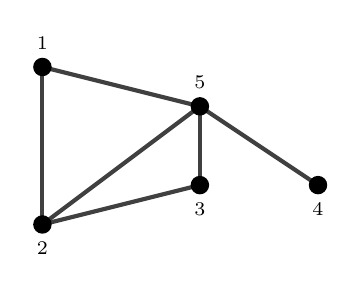
\begin{tikzpicture}
        \SetVertexStyle[FillColor=black, MinSize=0.7]
        \Vertex[x=0, y=0,IdAsLabel, position=below]{2}
        \Vertex[x=0, y=2, IdAsLabel, position=above]{1}
        \Vertex[x=2, y=1.5, IdAsLabel, position=above]{5}
        \Vertex[x=2, y=0.5, IdAsLabel, position=below]{3}
        \Vertex[x=3.5, y=0.5, IdAsLabel, position=below]{4}
        
        \Edge[](1)(2)
        \Edge[](2)(5)
        \Edge[](2)(3)
        \Edge[](1)(5)
        \Edge[](3)(5)
        \Edge[](4)(5)
        % \Edge[](3)(4)
        \end{tikzpicture}
\end{center}
 
\end{quest}

%%% TERMINA EL EJERCICIO 3 %%%

%%% EMPIEZA EL EJERCICIO 4 %%%


\begin{quest}\verb|[2 pts.]| Un grafo se dice "arco-circular" si es el grafo intersección de arcos abiertos alrededor de un círculo, es decir, si se pueden representar sus vértices a través de dichos arcos de modo de que cada intervalo está asociado a un vértice y dos vertices son adyacentes si y solo si los arcos se intersectan. Por ejemplo el siguiente grafo: 
\begin{center}
    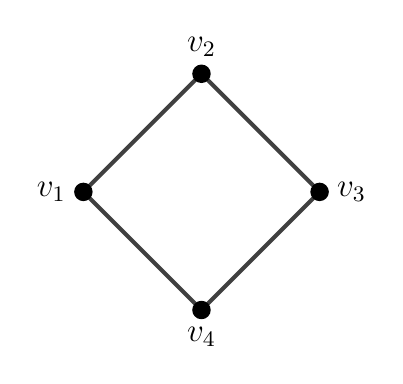
\begin{tikzpicture}
        \SetVertexStyle[FillColor=black, MinSize=0.7]
        \Vertex[label=$v_1$, position=left, fontsize=\large, x=0, y=0]{v1}
        \Vertex[label=$v_2$, position=above, fontsize=\large, x=1.5, y=1.5]{v2}
        \Vertex[label=$v_3$, position=right, fontsize=\large, x=3, y=0]{v3}
        \Vertex[label=$v_4$, position=below, fontsize=\large, x=1.5, y=-1.5]{v4}
        \Edge(v1)(v2)
        \Edge(v2)(v3)
        \Edge(v3)(v4)
        \Edge(v4)(v1)
    \end{tikzpicture}
\end{center}
es arco-circular porque tiene, entre otras, la siguiente representación en arcos:

\begin{center}
    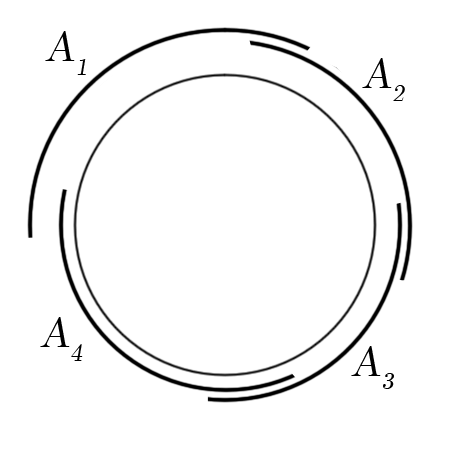
\includegraphics[scale=1.3]{../2021/Imagenes/arc.png}
\end{center}
% (dibujar A_1 que se interseque con A_2, A_2 con A_3. A_3 con A_4 y A_4 con A_1) 

\begin{enumerate}[label=\alph*)]
    \item Mostrar un grafo que no sea arco-circular. Justificar.
    \item Un grafo arco-circular es arco-circular-unitario, si existe una representación de modo que todos los arcos tengan la misma longitud. Mostrar que el siguiente grafo: 
    \begin{center}
        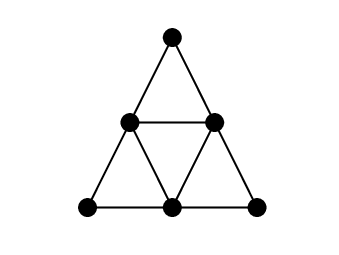
\includegraphics[]{../2021/Imagenes/The-Hajos-Graph.png}
    \end{center}
    es arco-circular pero NO es arco-circular-unitario.
\end{enumerate}
\end{quest}

%%% TERMINA EL EJERCICIO 4 %%%

%%% EMPIEZA EL EJERCICIO 5 %%%

\begin{quest} \verb|[2.5 pts.]| El 8-puzzle es un juego en el que a partir de un estado inicial se debe llegar al estado objetivo. Cada movimiento consiste en intercambiar el lugar de la ficha blanca con alguna de las fichas adyacentes que se encuentran arriba, abajo, a izquierda o a derecha. A continuación se muestran el estado objetivo y un ejemplo de estado inicial:

\begin{center}
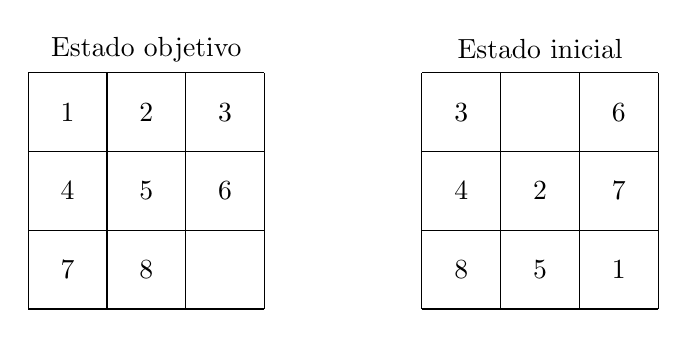
\begin{tikzpicture}
    \node at (1.5, 3.3) {Estado objetivo};
    \draw[step=1cm,black,thin] (0,0) grid (3,3);
    \node at (0.5,2.5) {1};
    \node at (1.5,2.5) {2};
    \node at (2.5,2.5) {3};
    \node at (0.5,1.5) {4};
    \node at (1.5,1.5) {5};
    \node at (2.5,1.5) {6};
    \node at (0.5,0.5) {7};
    \node at (1.5,0.5) {8};

    \node at (6.5, 3.3) {Estado inicial};
    \draw[step=1cm,black,thin] (5,0) grid (8,3);
    \node at (5.5, 0.5) {8};
    \node at (6.5, 0.5) {5};
    \node at (7.5, 0.5) {1};
    \node at (5.5, 1.5) {4};
    \node at (6.5, 1.5) {2};
    \node at (7.5, 1.5) {7};
    \node at (5.5, 2.5) {3};
    \node at (7.5, 2.5) {6};
\end{tikzpicture}
\end{center}
Modelar el problema de llegar desde un estado inicial al estado objetivo en la menor cantidad de movimientos como un problema de grafos y proponer un algoritmo que utilice dicho grafo para resolverlo en tiempo polinomial.
\end{quest}

%%% TERMINA EL EJERCICIO 4 %%%

%%% TERMINA EL PARCIAL %%%



\end{document}

